\documentclass{tufte-handout}

\title{CS224n: Natural Language Processing with Deep Learning\thanks{Course Instructors: Christopher Manning, Richard Socher}}

\author[Lisa Wang, Juhi Naik, Shayne Longpre]{Lecture Notes: Part IV\thanks{Authors: Lisa Wang, Juhi Naik, and Shayne Longpre}}

\date{Winter 2017} % without \date command, current date is supplied

%\geometry{showframe} % display margins for debugging page layout

\usepackage{graphicx} % allow embedded images
  \setkeys{Gin}{width=\linewidth,totalheight=\textheight,keepaspectratio}
  \graphicspath{{notes4/fig/}} % set of paths to search for images
\usepackage{amsmath}  % extended mathematics
\usepackage{amstext}  % extended text
\usepackage{booktabs} % book-quality tables
\usepackage{units}    % non-stacked fractions and better unit spacing
\usepackage{multicol} % multiple column layout facilities
\usepackage{lipsum}   % filler text
\usepackage{fancyvrb} % extended verbatim environments
\usepackage{placeins}
  \fvset{fontsize=\normalsize}% default font size for fancy-verbatim environments
\usepackage[normalem]{ulem}
\usepackage{algpseudocode}
\usepackage{algorithm}


% tikz package
\usepackage{tikz}
\usetikzlibrary{patterns, shapes,calc,positioning,arrows,mindmap,matrix}
\usetikzlibrary{decorations.pathreplacing}

% Standardize command font styles and environments
\newcommand{\doccmd}[1]{\texttt{\textbackslash#1}}% command name -- adds backslash automatically
\newcommand{\docopt}[1]{\ensuremath{\langle}\textrm{\textit{#1}}\ensuremath{\rangle}}% optional command argument
\newcommand{\docarg}[1]{\textrm{\textit{#1}}}% (required) command argument
\newcommand{\docenv}[1]{\textsf{#1}}% environment name
\newcommand{\docpkg}[1]{\texttt{#1}}% package name
\newcommand{\doccls}[1]{\texttt{#1}}% document class name
\newcommand{\docclsopt}[1]{\texttt{#1}}% document class option name
\newenvironment{docspec}{\begin{quote}\noindent}{\end{quote}}% command specification environment
\newcommand{\argmin}{\operatornamewithlimits{argmin}}
\newcommand{\argmax}{\operatornamewithlimits{argmax}}
\newcommand{\textunderscript}[1]{$_{\text{#1}}$}

\setcounter{secnumdepth}{3}

\begin{document}

\maketitle% this prints the handout title, author, and date

\textbf{Keyphrases: Dependency Parsing.}
%\printclassoptions
\section{Dependency Grammar and Dependency Structure}
Parse trees in NLP, analogous to those in compilers, are used to analyze the syntactic structure of sentences. There are two main types of structures used - constituency structures and dependency structures. 

Constituency Grammar uses phrase structure grammar to organize words into nested constituents. This will be covered in more detail in following chapters. We now focus on Dependency Parsing.

Dependency structure of sentences shows which words depend on (modify or are arguments of) which other words. These binary asymmetric relations between the words are called dependencies and are depicted as arrows going from the \textbf{head} (or governor, superior, regent) to the \textbf{dependent} (or modifier, inferior, subordinate). Usually these dependencies form a tree structure. They are often 	typed with the name of grammatical relations (subject, prepositional object, apposition, etc.). An example of such a dependency tree is shown in Figure~\ref{fig:dep_tree}. Sometimes a fake \textsc{ROOT} node is added as the head to the whole tree so that every word is a dependent of exactly one node.

\begin{marginfigure}
	\centering
	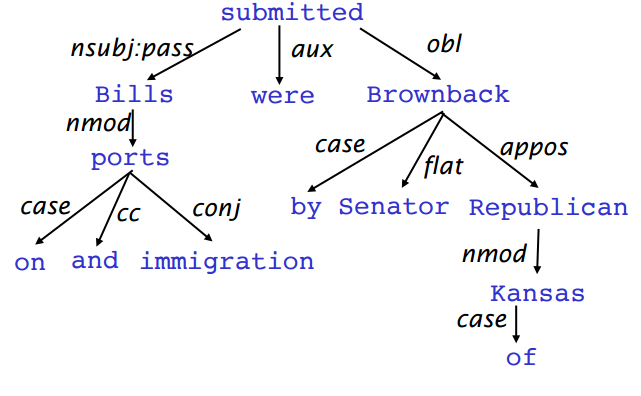
\includegraphics[width=\linewidth]{dep_tree.png}
	\caption {Dependency tree for the sentence "Bills on ports and immigration were submitted by Senator Brownback, Republican of Kansas"}
	\label{fig:dep_tree}
\end{marginfigure}

\subsection{Dependency Parsing}

Dependency parsing is the task of analyzing the syntactic dependency structure of a given input sentence $S$. The output of a dependency parser is a dependency tree where the words of the input sentence are connected by typed dependency relations. Formally, the dependency parsing problem asks to create a mapping from the input sentence with words $S=w_0w_1...w_n$ (where $w_0$ is the $\textsc{ROOT}$) to its dependency tree graph $G$. 
Many different variations of dependency-based methods have been developed in recent years, including neural network-based methods, which we will describe later.  \\
% they all have in common that they do not make any assumptions of the specific dependency types (e.g. grammatical functions). \\
To be precise, there are two subproblems in dependency parsing (adapted from Kuebler et al., chapter 1.2): 
\begin{enumerate}
\item \textit{Learning:}
Given a training set $D$ of sentences annotated with dependency graphs, induce a parsing model $M$ that can be used to parse new sentences.
\item \textit{Parsing:}
Given a parsing model $M$ and a sentence $S$, derive the optimal dependency graph $D$ for $S$ according to $M$.
\end{enumerate}


% copy over to references 
% @article{kubler2009dependency,
%   title={Dependency parsing},
%   author={K{\"u}bler, Sandra and McDonald, Ryan and Nivre, Joakim},
%   journal={Synthesis Lectures on Human Language Technologies},
%   volume={1},
%   number={1},
%   pages={1--127},
%   year={2009},
%   publisher={Morgan \& Claypool Publishers}
% }

\subsection{Transition-Based Dependency Parsing}
Transition-based dependency parsing relies on a state machine which defines the possible transitions to create the mapping from the input sentence to the dependency tree. 
The \textit{learning problem} is to induce a model which can predict the next transition in the state machine based on the transition history. The \textit{parsing problem} is to construct the optimal sequence of transitions for the input sentence, given the previously induced model.  
Most transition-based systems do not make use of a formal grammar.

\subsection{Greedy Deterministic Transition-Based Parsing}
%  using a greedy deterministic parsing algorithm.
This system was introduced by Nivre in 2003 and was radically different from other methods in use at that time.\\
This transition system is a state machine, which consists of \textit{states} and  \textit{transitions} between those states.  The model induces a sequence of transitions from some \textit{initial} state to one of several \textit{terminal} states.

\textbf{States: }\\
For any sentence $S=w_0w_1...w_n$, a state can be described with a triple $c=(\sigma, \beta, A)$:
\begin{enumerate}
\item a stack $\sigma$ of words $w_i$ from $S$,
\item a buffer $\beta$ of words $w_i$ from $S$,
\item  a set of dependency arcs $A$ of the form $(w_i, r, w_j)$, where $w_i, w_j$ are from $S$, and $r$ describes a dependency relation.
\end{enumerate}
It follows that for any sentence $S=w_0w_1...w_n$,
\begin{enumerate}
\item an \textit{initial} state $c_0$ is of the form  $([ w_0]_{\sigma}, [w_1, ...,w_n]_{\beta}, \emptyset)$ (only the $\textsc{ROOT}$ is on the stack $\sigma$, all other words are in the buffer $\beta$ and no actions have been chosen yet),
\item a terminal state has the form $(\sigma, []_{\beta}, A)$.
\end{enumerate}

\textbf{Transitions:} \\
% add image of transitions 

\begin{marginfigure}
	\centering
	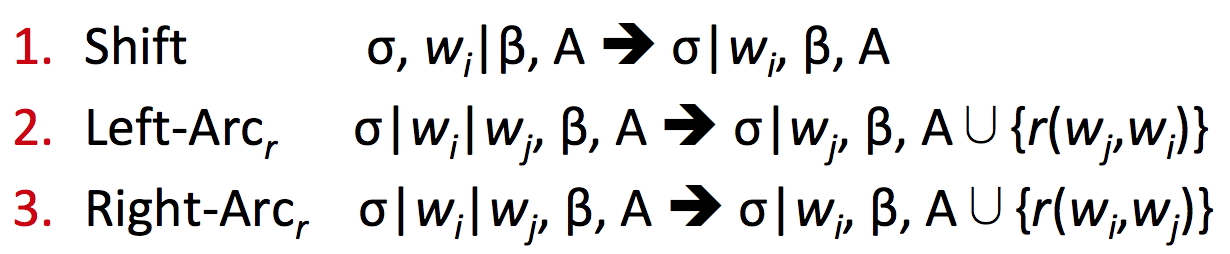
\includegraphics[width=\linewidth]{transitions}
  \caption{Transitions for Dependency Parsing.}
  \label{fig:transitions}
\end{marginfigure}

There are three types of transitions between states:
\begin{enumerate}
\item $\textsc{Shift}$:  Remove the first word in the buffer  and push it on top of the stack. (Pre-condition: buffer has to be non-empty.)
% \item  $\textsc{Left-Arc}_r$: Add a dependency arc $(w_j, r, w_i)$ to the arc set $A$, where $w_i$ is the word on the top of the stack and $w_j$ is the first word in the buffer. Pop $w_i$ of the stack. (Pre-condition: both the stack and the buffer have to be non-empty and $w_i$ cannot be the $\textsc{ROOT}$. )
% \item  $\textsc{Right-Arc}_r$:  Add a dependency arc $(w_i, r, w_j)$ to the arc set $A$, where $w_i$ is the word on the top of the stack and $w_j$ is the first word in the buffer. Pop $w_i$ of the stack. Replace $w_j$ with $w_i$ at the front of the buffer. (Pre-condition: both the stack and the buffer have to be non-empty.)
\item  $\textsc{Left-Arc}_r$: Add a dependency arc $(w_j, r, w_i)$ to the arc set $A$, where $w_i$ is the word second to the top of the stack and $w_j$ is the word at the top of the stack. Remove $w_i$ from the stack. (Pre-condition: the stack needs to contain at least two items and $w_i$ cannot be the $\textsc{ROOT}$.)
\item  $\textsc{Right-Arc}_r$:  Add a dependency arc $(w_i, r, w_j)$ to the arc set $A$, where $w_i$ is the word second to the top of the stack and $w_j$ is the word at the top of the stack. Remove $w_j$ from the stack.  (Pre-condition: The stack needs to contain at least two items.)
\end{enumerate}
A more formal definition of these three transitions is presented in Figure ~\ref{fig:transitions}.

\subsection{Neural Dependency Parsing}

While there are many deep models for dependency parsing, this section focuses specifically on greedy, transition-based neural dependency parsers. This class of model has demonstrated comparable performance and significantly better efficiency than traditional feature-based discriminative dependency parsers. The primary distinction from previous models is the reliance on dense rather than sparse feature representations.

The model we will describe employs the arc-standard system for transitions, as presented in section 1.3. Ultimately, the aim of the model is to predict a transition sequence from some initial configuration $c$ to a terminal configuration, in which the dependency parse tree is encoded. As the model is greedy, it attempts to correctly predict one transition $T\in\{\textsc{shift},\textsc{Left-Arc}_r,\textsc{Right-Arc}_r\}$ at a time, based on features extracted from the current configuration $c=(\sigma, \beta, A)$. Recall, $\sigma$ is the stack, $\beta$ the buffer, and $A$ the set of dependency arcs for a given sentence.
\par% or empty line in the source code
\bigskip
\textbf{Feature Selection:}
\par% or empty line in the source code
\bigskip

Depending on the desired complexity of the model, there is flexibility in defining the input to the neural network. The features for a given sentence $S$ generally include some subset of:

\begin{enumerate}
\item $S_{word}$: Vector representations for some of the words in $S$ (and their dependents) at the top of the stack $\sigma$ and buffer $\beta$.
\item $S_{tag}$: Part-of-Speech (POS) tags for some of the words in $S$. POS tags comprise a small, discrete set: $\mathcal{P}=\{NN,NNP,NNS,DT,JJ,...\}$ 
\item $S_{label}$: The arc-labels for some of the words in $S$. The arc-labels comprise a small, discrete set, describing the dependency relation: $\mathcal{L}=\{amod,tmod,nsubj,csubj,dobj,...\}$
\end{enumerate}
For each feature type, we will have a corresponding embedding matrix, mapping from the feature's one hot encoding, to a $d$-dimensional dense vector representation. The full embedding matrix for $S_{word}$ is $E^w \in \mathbb{R}^{d \times N_w}$ where $N_w$ is the dictionary/vocabulary size. Correspondingly, the POS and label embedding matrices are $E^t \in \mathbb{R}^{d \times N_t}$ and $E^l \in \mathbb{R}^{d \times N_l}$ where $N_t$ and $N_l$ are the number of distinct POS tags and arc labels. \\
Lastly, let the number of chosen elements from each set of features be denoted as $n_{word}$, $n_{tag}$, and $n_{label}$ respectively. \\

\par% or empty line in the source code
\bigskip
\textbf{Feature Selection Example:}
\par% or empty line in the source code
\bigskip

As an example, consider the following choices for $S_{word}$, $S_{tag}$, and $S_{label}$.
\begin{enumerate}
\item $S_{word}$: The top 3 words on the stack and buffer: $s_1, s_2, s_3, b_1, b_2, b_3$. The first and second leftmost / rightmost children of the top two words on the stack: $lc_1(s_i), rc_1(s_i), lc_2(s_i), rc_2(s_i)$, $i = 1, 2$. The leftmost of leftmost / rightmost of rightmost children of the top two words on the stack: $lc_1(lc_1(s_i)), rc_1(rc_1(s_i))$, $i = 1, 2$. In total $S_{word}$ contains $n_w = 18$ elements.
\item $S_{tag}$: The corresponding POS tags for $S_{tag}$ ($n_t = 18$).
\item $S_{label}$: The corresponding arc labels of words, excluding those 6 words on the stack/buffer ($n_l = 12$).
\end{enumerate}
Note that we use a special $\textsc{Null}$ token for non-existent elements: when the stack and buffer are empty or dependents have not been assigned yet. For a given sentence example, we select the words, POS tags and arc labels given the schematic defined above, extract their corresponding dense feature representations produced from the embedding matrices $E^w$, $E^t$, and $E^l$, and concatenate these vectors into our inputs $[x^{w},x^{t},x^{l}]$. At training time we backpropagate into the dense vector representations, as well as the parameters at later layers.

\par% or empty line in the source code
\bigskip
\textbf{Feedforward Neural Network Model:}
\par% or empty line in the source code
\bigskip

The network contains an input layer $[x^{w},x^{t},x^{l}]$, a hidden layer, and a final softmax layer with a cross-entropy loss function. We can either define a single weight matrix in the hidden layer, to operate on a concatenation of $[x^{w},x^{t},x^{l}]$, or we can use three weight matrices $[W_{1}^{w},W_{1}^{t},W_{1}^{l}]$, one for each input type, as shown in Figure ~\ref{fig:model_arch}. We then apply a non-linear function and use one more affine layer $[W_{2}]$ so that there are an equivalent number of softmax probabilities to the number of possible transitions (the output dimension).

\begin{figure*}[!ht]
	% \ifx \allfiles \undefined

% \documentclass{article}

% \usepackage{tikz}
% \usetikzlibrary{shapes,calc,positioning,arrows,mindmap,matrix}
% \usetikzlibrary{decorations.pathreplacing}

% \begin{document}
% \fi

\def\layersep{1.2cm}
\def\numHidden{6}
\def\numOutput{4}
\def\dx{3.3}
\def\dy{2.2}
\tikzset{
      treenode/.style = {align=center, inner sep=4pt, text centered,font=\sffamily},
    node/.style = {treenode, minimum width=1.3em, text height=1em},
	line/.style = {very thick, dashed, rounded corners, fill=orange!15!white, fill opacity=0.2}
}

% \tikzset{

%   line/.style = {very thick, dashed, fill=orange!30!white, fill opacity=0.2}
% }

\begin{tikzpicture}[scale=0.8,shorten >=1pt,->,draw=black!50, node distance=\layersep]

    \tikzstyle{neuron}=[circle,fill=black!25,minimum size=13pt,inner sep=0pt]
    \tikzstyle{annot} = [text width=15em, text centered]

    \foreach \name / \y in {1,...,3}
        \node[neuron,fill=red!50] (I-\name) at (\y/2, 0) {};

    \node[annot] (cdot-1) at (3/2+0.8,0) {$\cdots$};

    \foreach \name / \y in {4,...,6}
        \node[neuron,fill=red!50] (I-\name) at (\y/2+1, 0) {};

    \foreach \name / \y in {7,...,9}
        \node[neuron,fill=blue!50,postaction={pattern=north east lines}] (I-\name) at (\y/2+1.5, 0) {};

    \node[annot] (cdot-2) at (9/2+2.3,0) {$\cdots$};

    \foreach \name / \y in {10,...,12}
        \node[neuron,fill=blue!50,postaction={pattern=north east lines}] (I-\name) at (\y/2+2.5, 0) {};

    \foreach \name / \y in {13,...,15}
        \node[neuron,fill=orange!50,postaction={pattern=north west lines}] (I-\name) at (\y/2+3, 0) {};

    \foreach \name / \y in {1,...,3}
        \node[neuron,fill=gray!50] (H-\name) at (\y*0.8+2.4,\layersep) {};

    \node[annot] (cdot-3) at (5.5,\layersep) {$\cdots$};

    \foreach \name / \y in {4,...,6}
        \node[neuron,fill=gray!50] (H-\name) at (\y*0.8+3.1,\layersep) {};


    \foreach \name / \y in {1,...,2}
        \node[neuron,fill=black!50] (S-\name) at (\y*0.8+3.1,\layersep*2) {};

    \node[annot] (cdot-4) at (5.5,\layersep*2) {$\cdots$};

    \foreach \name / \y in {3,...,4}
        \node[neuron,fill=black!50] (S-\name) at (\y*0.8+3.8,\layersep*2) {};


     \foreach \source in {2,5,8,11,14}
	    \foreach \dest in {2, 5}
            \path (I-\source) edge (H-\dest);

    \foreach \source in {2, 5}
        \foreach \dest in {1,...,\numOutput}
            \path (H-\source) edge (S-\dest);

    
    \node[annot] at (-3,0) {\textbf{Input layer}: $[x^w, x^t, x^l]$};
    \node[annot] at (-3,\layersep){\textbf{Hidden layer}: \\ $h = (W^w_1 x^w + W^t_1 x^t + W^l_1 x^l + b_1)^3$};
    \node[annot] at (-3,\layersep*2){\textbf{Softmax layer}: \\ $p = \texttt{softmax}(W_2 h)$};

    \draw [line] ($(I-1.south west)+(-0.2, -0.2)$) rectangle ($(I-3.north east)+( 0.2, 0.2)$);
    \draw [line] ($(I-4.south west)+(-0.2, -0.2)$) rectangle ($(I-6.north east)+( 0.2, 0.2)$);
    \draw [line] ($(I-7.south west)+(-0.2, -0.2)$) rectangle ($(I-9.north east)+( 0.2, 0.2)$);
    \draw [line] ($(I-10.south west)+(-0.2, -0.2)$) rectangle ($(I-12.north east)+( 0.2, 0.2)$);
    \draw [line] ($(I-13.south west)+(-0.2, -0.2)$) rectangle ($(I-15.north east)+( 0.2, 0.2)$);

   	\draw [line,solid] ($(I-1.south west)+(-0.3, -0.3)$) rectangle ($(I-15.north east)+( 0.3, 0.3)$);

   	\draw [line,solid] ($(H-1.south west)+(-0.2, -0.2)$) rectangle ($(H-\numHidden.north east)+( 0.2, 0.2)$);
    \draw [line,solid] ($(S-1.south west)+(-0.3, -0.3)$) rectangle ($(S-\numOutput.north east)+( 0.3, 0.3)$);

    \draw [decorate,decoration={brace,amplitude=5pt,mirror,raise=3pt}] ($(I-1.south west)+(-0.3, -0.3)$) -- ($(I-6.south east)+(0.3, -0.3)$) node [black,midway,yshift=-0.6cm] {words};

    \draw [decorate,decoration={brace,amplitude=5pt,mirror,raise=3pt}] ($(I-7.south west)+(-0.3, -0.3)$) -- ($(I-12.south east)+(0.3, -0.3)$) node [black,midway,yshift=-0.6cm] {POS tags};

    \draw [decorate,decoration={brace,amplitude=5pt,mirror,raise=3pt}] ($(I-13.south west)+(-0.3, -0.3)$) -- ($(I-15.south east)+(0.3, -0.3)$) node [black,midway,yshift=-0.6cm] {arc labels};


\node [node] at (-2+\dx,-5+\dy) (1) {ROOT};

\node [node] at (0+\dx,-5+\dy) (2) {has\_VBZ}
child[level distance=1.25cm]
{ 
node [node,xshift=-1cm,font=\sffamily] (4) {He\_PRP}
edge from parentnode[left, xshift=1.3cm, yshift=-0.2cm] {nsubj}
};

\node [node] at (0+\dx,-5+\dy) (2) {has\_VBZ};
\node [node] at (2+\dx,-5+\dy) (3) {good\_JJ};
\node [node] at (5+\dx,-5+\dy) (4) {control\_NN};
\node [node] at (7+\dx,-5+\dy) (5) {.\_.};

\node [node] at (0+\dx,-4+\dy) {Stack};
\node [node] at (6+\dx,-4+\dy) {Buffer};

% \path (3) edge (I-5);
% \path (3) edge (I-8);

% \draw [dashed, thick, ->] (2+\dx,-4.8+\dy) -- (3.5,-0.2);
% \draw [dashed, thick, ->] (2.5+\dx,-4.8+\dy) -- (5.5,-0.2);
% \draw [dashed, thick, ->] (0.5+\dx,-5.8+\dy) -- (10,-0.2);

\node[annot] at (-3,-5+\dy){\textbf{Configuration}};

\draw [very thick, fill=orange!30!white, fill opacity=0.2] ($(1.south west)+(-0.1, -0.1)$) rectangle ($(3.north east)+( 0.1, 0.1)$);
\draw [very thick, fill=orange!30!white, fill opacity=0.2] ($(4.south west)+(-0.1, -0.1)$) rectangle ($(5.north east)+( 0.1, 0.1)$);

\end{tikzpicture}
% End of code

% \ifx \allfiles \undefined
% \end{document}
% \fi

	\caption{The neural network architecture for greedy, transition-based dependency parsing.}
	\label{fig:model_arch}
\end{figure*}

Note that in Figure ~\ref{fig:model_arch}, $f(x)=x^3$ is the non-linear function used.

\par% or empty line in the source code
\bigskip
For a more complete explanation of a greedy transition-based neural dependency parser, refer to "A Fast and Accurate Dependency Parser using Neural Networks" under Further Reading.

\par% or empty line in the source code
\bigskip

\textbf{Further reading:} \\

Danqi Chen, and Christopher D. Manning. "A Fast and Accurate Dependency Parser using Neural Networks." EMNLP. 2014. \\

Kuebler, Sandra, Ryan McDonald, and Joakim Nivre. ``Dependency parsing.'' Synthesis Lectures on Human Language Technologies 1.1 (2009): 1-127.

\end{document}